\documentclass[10pt,a4paper]{article}
\usepackage[margin=22mm]{geometry}
\usepackage[T1]{fontenc}
\usepackage{lmodern,microtype}
\usepackage{amsmath,amssymb,graphicx,booktabs,array,longtable}
\usepackage{xcolor,hyperref,fancyhdr}
\usepackage[section]{placeins}
\definecolor{ink}{HTML}{173E66}
\hypersetup{colorlinks=true,linkcolor=ink,urlcolor=ink,citecolor=ink,pdftitle={Diffusion-Lagr: Bounded Reproduction Audit and Numerical Validation}}
\pagestyle{fancy}\fancyhf{}
\fancyhead[L]{\small Diffusion-Lagr: bounded reproduction audit}
\fancyhead[R]{\small 26 October 2026}
\fancyfoot[L]{\footnotesize Demo validation and analytic recalculation; not full reproduction}
\fancyfoot[R]{\thepage}
\setlength{\headheight}{14pt}
\setlength{\parindent}{0pt}\setlength{\parskip}{5pt}
\setlength{\emergencystretch}{2em}
\widowpenalty=10000\clubpenalty=10000
\newcolumntype{L}[1]{>{\raggedright\arraybackslash}p{#1}}
\newcommand{\RoundTripError}{5.3291\times10^{-15}}
\newcommand{\DenseSeconds}{16.82}
\newcommand{\ExploreSeconds}{17.22}
\newcommand{\DenseDifference}{0.01617}
\newcommand{\SparseDifference}{2.23469}
\newcommand{\SampleToPhysicalFactor}{1.9753\times10^{5}}

\title{\color{ink}Synthetic Lagrangian Turbulence\\[4pt]\large Reproduction audit, numerical validation, and estimator exploration}
\author{Reproducible research workbench for JackYansongLi}
\date{26 October 2026\quad |\quad Bounded one-hour deliverable}
\begin{document}
\maketitle
\begin{center}
\fcolorbox{ink}{blue!3}{\begin{minipage}{0.92\linewidth}
\textbf{Completion statement.} This report contains measured results on the repository's 256-trajectory DNS demo, numerical tests, and recalculated analytic noise schedules. It does \textbf{not} claim reproduction of all paper figures, full-data model statistics, trained model quality, or rare-event generalization. No neural model was trained or sampled. All missing dependencies and unrun panels remain explicit.
\end{minipage}}
\end{center}

\begin{abstract}
We establish a reproducible starting point for the study by Li et al.\ \cite{li2024}, pin its source revision, audit the experimental dependencies, and execute a bounded set of real-data and analytic checks. The requested fork is created in the verified GitHub account and experimental work is isolated on a research branch. The bundled one- and three-component datasets are shown to encode the same 256 physical trajectories, with inverse-normalization agreement to floating-point precision. A trajectory-cluster bootstrap gives uncertainty conditional on this small DNS subset. Explicit derivative conventions reconcile otherwise incompatible acceleration scales. The published and implemented linear diffusion schedules differ, while the tanh and power schedules agree up to terminal clipping and floating-point error. Original finite-subset and estimator-sensitivity experiments reveal severe concentration of high-order moments and noisy long-lag local exponents. These findings motivate a staged full-data reanalysis and efficient checkpoint sampling, rather than a claim of improved generative-model performance.
\end{abstract}

\section{Scope, provenance, and evidence classes}
The target is \textbf{arXiv:2307.08529v2}, revised 28 April 2024, including its separate Supplementary Information. The requested repository is itself a fork of the authors' SmartTURB repository. The newly created fork is
\href{https://github.com/JackYansongLi/diffusion-lagr}{JackYansongLi/diffusion-lagr}, with direct parent \texttt{leopc999/diffusion-lagr} and upstream commit
\begin{quote}\small\texttt{77da6cdc67775aa45af6c4148068f00a75e54c41}.\end{quote}
The working branch is \texttt{research/reproduction-audit-20261026}. Original training and sampling code is preserved; additions reside in \texttt{repro/}. No existing user work was overwritten. Authenticated account checks used the GitHub connector and a network-enabled CLI identity read; credentials are not stored in the report.

Four evidence classes are kept separate: (i) analytic recalculation from equations and code; (ii) measured pipeline validation on the bundled DNS demo; (iii) future reanalysis of author-generated trajectories; and (iv) future independent model sampling or retraining. Only the first two were executed. The exploration in Section~\ref{sec:explore} is a new analysis of estimator behavior, not a new model.

\section{Assets, figure inventory, and feasibility}
The migrated public record\ \cite{data} contains DNS data, author-generated samples, and demo files. Its DOI metadata was verified by the independent paper audit. Local MD5 checks reproduce both published demo checksums. Large assets were not downloaded under the one-hour constraint.

\begin{table}[ht]
\centering\small
\begin{tabular}{L{64mm}rr}
\toprule Asset & Decimal GB & Local status\\\midrule
DNS: 327680 trajectories, $2000\times3$, float64 & 15.729 & Not downloaded\\
DNS one-component concatenation & 15.729 & Not downloaded\\
Author DM-1c: $358400\times2000\times1$ & 2.867 & Not downloaded\\
Author DM-3c: $358400\times2000\times3$ & 8.602 & Not downloaded\\
Bundled DNS3c demo: $256\times2000\times3$ & 0.0123 & Measured\\
Bundled DNS1c demo: $768\times2000\times1$ & 0.0123 & Measured\\
\bottomrule
\end{tabular}
\caption{Public data inventory. DNS1c is redundant for analysis if DNS3c and its normalization are available. Exact filenames, byte counts, MD5s and URLs are in \texttt{repro/manifests/assets.json}. Data attribution: Li et al., CC-BY-4.0\ \cite{data}.}
\end{table}

The DNS3c file plus both published model sample arrays total 27.197 GB; extracting the NPZ arrays for memory mapping adds about 11.469 GB. A practical workspace should reserve at least 50 GB. The paper's extreme-tail sample counts are substantially larger than the available 358400-sample archives. Depending on how the paper's reference trajectory count treats component pooling, 86 times 327680 scalar records already requires approximately 225.4 GB in float32; 22 times requires 57.7 GB. These are lower interpretation-dependent storage estimates, not completed acquisitions.

The Mac has an M1 Pro, eight CPU cores, a 14-core integrated GPU, 16 GiB unified memory and approximately 729 GiB free storage at audit. It has no CUDA device. The existing Python analysis environment and HDF5 CLI were reused. The author's A100 training environment is not recreated. The paper reports about 25 hours for DM-1c and 40 hours for DM-3c on four A100s, or approximately 100 and 160 A100 GPU-hours. Its sampling example is also costly\ \cite{li2024}; no unmeasured throughput extrapolation to this Mac is made.

\small
\begin{longtable}{L{15mm}L{47mm}L{85mm}}
\caption{Every main and supplementary panel has a status. ``Unrun'' never means a failed numerical agreement test.}\label{tab:inventory}\\
\toprule Panel(s) & Required observation & Status and blocker\\\midrule
\endfirsthead
\toprule Panel(s) & Required observation & Status and blocker\\\midrule
\endhead
1a & Increment densities, including reduced-data model & Unrun. DNS, full DM-1c and 10\% model needed; archive sample count does not match the paper's 86-fold tail ensemble.\\
1b--d & Single-component trace examples & Unrun. Author DM-1c samples or new checkpoint samples needed.\\
1e--f & Three-component traces and integrated paths & Unrun. DNS and DM-3c needed; selection and integration conventions must be stated.\\
2 main & Acceleration density & Unrun. Includes missing 10\% model. Derivative convention audited, not inferred silently.\\
2 inset & Acceleration correlation & Unrun. Needs corresponding DNS/DM ensembles and derivative units.\\
3a & Architecture and hyperparameters & Documented from code/configs; no neural forward pass executed.\\
3b & Noise schedules & Analytic recalculation complete, with paper and upstream linear variants separately identified.\\
3c--f & Statistics and trajectories along reverse sampling & Unrun. Needs DM-1c checkpoint and states $V_{416},V_{216},V_{48},V_0$. New selective-history sampler is provided but not executed.\\
4a & Structure functions, orders 2, 4, 6 & Unrun paper comparison. Statistical kernel validated on demo; full DNS/DM reanalysis pending.\\
4b & Generalized flatness, orders 4, 6, 8 & Same status; high-order demo estimates are demonstrably fragile.\\
4c & Mixed component flatness & Unrun full comparison. Three-component kernel tested.\\
5a & Local fourth-order exponent & Unrun full comparison. Dense-lag estimator sensitivity measured on demo only.\\
5b & External DNS/experiment compilation & External data missing. The paper redraws Arneodo et al.\ \cite{arneodo}; copied or digitized curves would not be a rerun.\\
6 main & Training-loss history & Full history absent; no retraining attempted.\\
6 inset & Checkpoint-stage flatness & 10k and 30k checkpoints absent; final pretrained model alone is insufficient.\\
S1a--b & Reduced-training-data comparison & 1\% and 10\% assets absent.\\
S2a--b & WGAN comparison & WGAN code/checkpoint/samples absent from the specified repository.\\
\bottomrule
\end{longtable}
\normalsize
The supplementary inventory follows the independent paper audit. The machine-readable panel registry is \texttt{repro/manifests/figures.json}. No missing panel is replaced with a Gaussian proxy, a copied image, or an unlabeled demo plot.

\section{Numerical definitions and uncertainty}
Let $u_{r,k,i}$ denote component $i$ of physical trajectory $r$ at time sample $k$ after reversing the provided normalization,
\begin{equation}
u=(\tilde u+1)(u_{\max}-u_{\min})/2+u_{\min}.
\end{equation}
For integer lag $\ell$, $\delta_\ell u_{r,k,i}=u_{r,k+\ell,i}-u_{r,k,i}$. All reductions use float64. The kernels compute per-trajectory, per-component sufficient statistics before aggregating:
\begin{align}
S_p(\ell)&=\langle(\delta_\ell u)^p\rangle,&
F_p(\ell)&=S_p(\ell)/S_2(\ell)^{p/2},\\
F_{4,\mathrm{mixed}}(\ell)&=\frac{\frac13\sum_{i<j}\langle(\delta_\ell u_i)^2(\delta_\ell u_j)^2\rangle}{S_2(\ell)^2},&
\zeta_p(\ell)&=\frac{d\log S_p/d\log\ell}{d\log S_2/d\log\ell}.
\end{align}
The mixed denominator uses the pooled second moment, matching the paper's definition. Histograms divide counts by the total sample count and bin width, retain excluded-tail counts, and never silently renormalize a truncated tail.

The paper's min--max error representation uses ten trajectory partitions per component. Our corresponding envelope uses a recorded random partition and is \emph{not} a confidence interval. For three-component data, the 30 component-partitions do not create 30 independent DNS realizations. An additional percentile bootstrap resamples entire physical trajectories and keeps all time points and components together. Its 95\% intervals are conditional on exchangeability of these observed traces. They exclude shared-flow correlations, DNS-to-DNS variability, model training-seed uncertainty and discretization uncertainty. We do not resample correlated time samples as if they were independent.

The single-time quantities are computed from global pooled moments, not by averaging within-trajectory covariances:
\begin{equation}
E=\frac13\sum_i\langle u_i^2\rangle,\qquad
\Sigma^V=\frac13\sum_{i<j}\left[\langle u_i^2u_j^2\rangle-\langle u_i^2\rangle\langle u_j^2\rangle\right].
\end{equation}
The same definitions applied to acceleration yield $A$ and $\Sigma^A$. Each bootstrap replicate recomputes the pooled products and covariances.

\section{Measured demo validation and the acceleration-unit issue}
The one-component demo is exactly the component-wise concatenation of the three-component demo after inverse normalization, with maximum absolute difference $\RoundTripError$. Thus 768 scalar records represent only 256 physical trajectory clusters. Treating them as 768 independent samples would understate uncertainty.

\begin{table}[ht]
\centering\small
\begin{tabular}{lrrr}
\toprule Quantity & Demo estimate & Conditional 95\% interval & Paper DNS value\\\midrule
\csname @@input\endcsname single_time_table.tex
\bottomrule
\end{tabular}
\caption{Measured demo statistics and a reference comparison, not a full reproduction of Table II. Intervals use 2000 trajectory bootstrap resamples with seed 20261026. Acceleration uses \texttt{np.gradient} with sample spacing 1 and first-order one-sided boundary differences.}
\label{tab:single}
\end{table}

The demo's velocity-square cross covariance differs materially from the published full-data value; the latter also falls outside this conditional bootstrap interval. This is not evidence that the paper is wrong: the demo is a small, potentially nonrepresentative subset and all traces share a DNS realization. Agreement of the other rounded values does not establish reproduction of the full table.

The paper's physical sampling interval is $\Delta t_s=0.00225$ and its nominal dissipative scale is $\tau_\eta=0.021$. Their ratio is 9.333 samples per dissipative time; ``10 samples'' is an approximation. With the reported uncertainty $\tau_\eta=0.021\pm0.002$, this ratio spans approximately 8.44--10.22. We retain the explicit physical values rather than force numerical agreement through unit selection.

\begin{table}[ht]
\centering\small
\begin{tabular}{lrr}
\toprule Derivative convention & $A$, unit sample spacing & $A$, physical spacing\\\midrule
\csname @@input\endcsname derivative_table.tex
\bottomrule
\end{tabular}
\caption{Boundary handling and units are both explicit. Central interior differences use 1998 times, forward differences use 1999, and the NumPy-gradient convention uses all 2000.}
\end{table}

Changing the derivative's spacing from 1 to $0.00225$ multiplies $A$ by $\Delta t_s^{-2}=\SampleToPhysicalFactor$ and $\Sigma^A$ by $\Delta t_s^{-4}$. The demo values using sample-index derivatives round to the paper's acceleration entries. This is strong \emph{evidence for a unit-convention hypothesis}, not proof of the authors' exact implementation. Forward differences change $A$ by about 1.05\% relative to the all-point gradient; dropping endpoints explains the smaller difference between 329.33 and 329.61 in physical units. Standardizing a density removes a constant unit factor but not differences in the derivative stencil.

\begin{figure}[ht]
\centering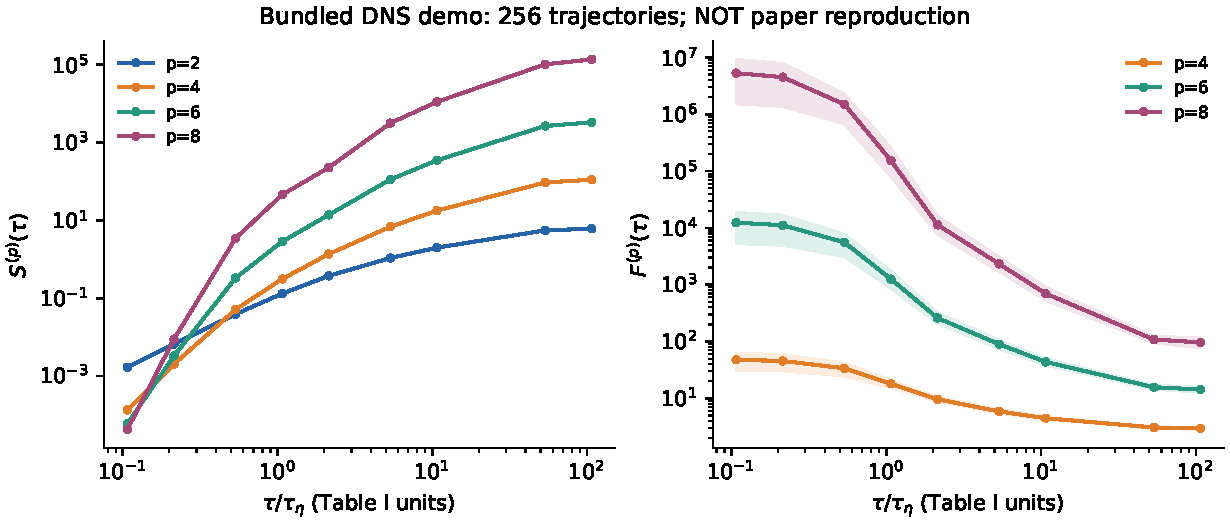
\includegraphics[width=\linewidth]{../repro/figures/demo_diagnostics.pdf}
\caption{Real bundled-DNS diagnostics. There are no diffusion-model curves. Shading is a conditional 400-resample trajectory-bootstrap interval; it is not the paper's error representation. Sparse lags are used here for a fast pipeline check, not for a publication local-slope comparison.}
\end{figure}

\section{Analytic schedule recalculation}
We evaluate the normalized tanh and power functions and their discrete beta sequences independently, then compare with the two original NumPy schedule functions extracted from the pinned source. No PyTorch import or proxy trajectory is needed for this check:
\begin{equation}
\bar\alpha(t)=\frac{-\tanh(7t-6)+\tanh(1)}{\tanh(6)+\tanh(1)},\qquad
\bar\alpha_{\mathrm{power4}}(t)=1-t^4,
\quad\beta_n=\min\!\left(1-\frac{\bar\alpha(n/N)}{\bar\alpha((n-1)/N)},0.999\right).
\end{equation}
For the tanh schedule, the largest beta discrepancy with upstream is approximately $3.11\times10^{-15}$. The discrete cumulative product agrees with the analytic function to approximately $1.73\times10^{-18}$ before the clipped final point. Terminal beta clipping leaves a small positive cumulative alpha instead of exactly zero.

\begin{figure}[ht]
\centering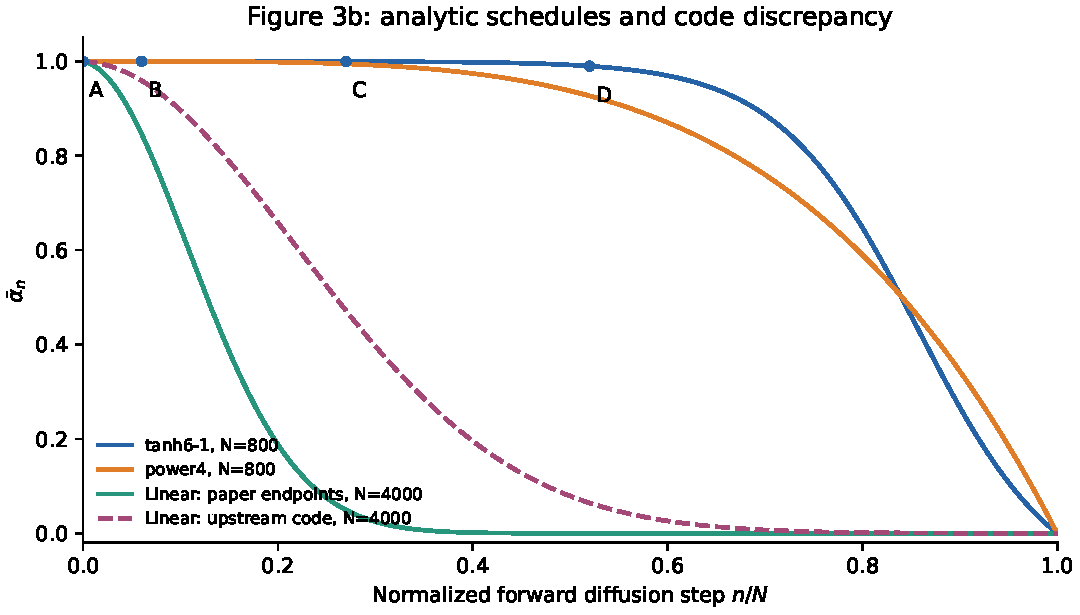
\includegraphics[width=.94\linewidth]{../repro/figures/figure3b_schedule_audit.pdf}
\caption{Recalculated Figure 3b schedule variants, displaying $1-\bar\alpha_n$ on a logarithmic ordinate. At $N=4000$, the paper states linear endpoints $10^{-4}$ and $0.02$; upstream scales both by $1000/N$, producing $2.5\times10^{-5}$ and $0.005$. Both are displayed. Labels A--D identify the published remaining-step fractions; A has zero noise and is annotated outside the log curve. No reverse trajectory was sampled.}
\end{figure}

\begin{table}[ht]
\centering\small
\begin{tabular}{lrrrr}
\toprule Variant & $N$ & First $\beta$ & Last $\beta$ & Terminal $\bar\alpha$\\\midrule
\csname @@input\endcsname schedule_table.tex
\bottomrule
\end{tabular}
\caption{Measured schedule endpoints. The code/paper linear discrepancy is unresolved provenance, not a reason to silently alter the baseline.}
\end{table}

\section{Original exploration: finite-sample and estimator sensitivity}\label{sec:explore}
This small experiment tests which conclusions the demo can support. For sizes 16, 32, 64, 128 and 256, we draw 200 subsets without replacement from the 256 physical trajectories, using seed 20261026. We recompute structure functions and normalize them by the estimate from the full demo. The resulting variation is conditional on this finite dataset; the full-demo estimate is not a known population truth.

\begin{table}[ht]
\centering\small
\begin{tabular}{rrrrr}
\toprule Order & CV, $n=16$, lag 10 & CV, $n=128$, lag 10 & Top 3 share, lag 1 & Max leave-one-out change, lag 1\\\midrule
\csname @@input\endcsname sensitivity_table.tex
\bottomrule
\end{tabular}
\caption{High-order moment concentration. CV is across repeated subsets. The top-three statistic ranks trajectories separately for each moment order; it is not a common set of three trajectories across all columns.}
\end{table}

At lag one, three of 256 trajectories contribute about 79\% of the eighth moment. Removing a single trajectory can alter its estimate by about 37\%. At lag ten, the eighth-moment subset CV is about 120\% for 16 traces and 29\% for 128, while the corresponding second-moment CVs are about 18\% and 4\%. These measured diagnostics explain why a visually plausible high-order demo curve is insufficient evidence of convergence. Rare trajectories are part of the scientific target; trimming them would change the estimand, so no trimmed result is substituted for the original moment.

We also compute $S_2$ and $S_4$ on all integer lags 1--1024 and compare second-order derivatives on the log-lag grid against a central-secant derivative ratio. Their maximum interior difference is $\DenseDifference$. Replacing the dense grid with a sparse grid changes local exponents at common lag points by up to $\SparseDifference$, dominated by the noisy large-lag regime where the second-moment derivative is small. This is a ratio-conditioning problem as well as a grid issue. These excursions must not be mistaken for model physics or smoothed away without disclosure.

\begin{figure}[ht]
\centering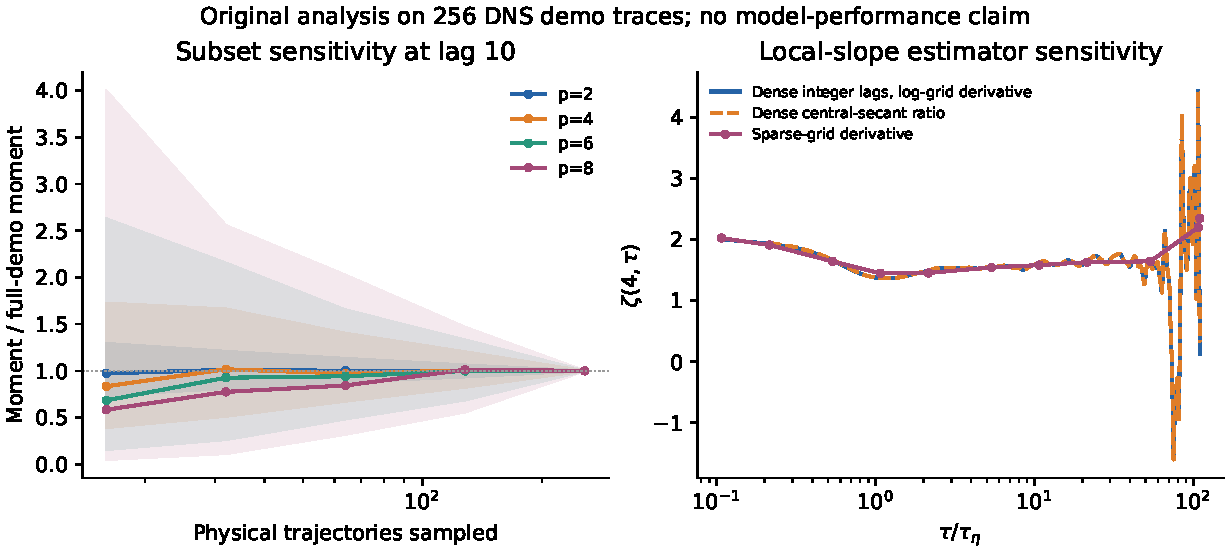
\includegraphics[width=\linewidth]{../repro/figures/demo_estimator_sensitivity.pdf}
\caption{New estimator study on measured demo data. Left: median and 5--95\% subset ranges at lag ten. Right: local-exponent sensitivity using the same data and explicit derivative conventions. These are neither confidence bands for the turbulence population nor a model-performance improvement.}
\end{figure}
The dense-grid calculation took \DenseSeconds\ seconds in the measured run; the numerical experiment before plotting took \ExploreSeconds\ seconds. This is a bounded CPU benchmark of the analysis code, not an estimate of neural sampling speed.

\section{Implementation, tests, and remaining experiments}
Nineteen numerical tests pass. They check exact polynomial-signal structure functions, Gaussian analytic moments, affine normalization, component permutation, mixed moments, squared covariance scaling, derivative time units, central differences, correlation at zero lag, histogram tail accounting, trajectory-chunk equivalence, bootstrap cluster preservation, input guards, upstream schedule equivalence, schedule clipping, rank-disjoint sample coverage and selected history indices. Artificial Gaussian signals are used solely as analytic-reference tests, never as turbulence reproduction data.

A separate read-only audit of the first published workbench commit, \texttt{47b024b}, reran all 19 tests and the Torch-free sampler plan. Its independently recomputed recorded numerical summaries agree at relative tolerance $10^{-14}$; sufficient statistics differ by at most $4.74\times10^{-16}$ relatively. The auditor also checked recorded source/output hashes. That review identified the Figure 3b ordinate as $1-\bar\alpha$ on a log scale; the plot and its output manifest were regenerated accordingly. This is independent validation of the bounded numerical work, not validation of neural inference or of full-paper results.

The original sampler aggregates all generated trajectories in memory on every rank. The new opt-in sampler writes one batch per shard and stores only requested reverse states. At $N=800$, retaining four states instead of 801 reduces trajectory-history storage by a factor of about 200, before temporary tensors. It records model/config hashes, effective arguments, unique global-batch seeds, per-shard output hashes and timings. It refuses existing rank outputs. Its plan and index logic are tested; \textbf{the neural execution path is not runtime-tested}, because this environment lacks the selected PyTorch model stack and no checkpoint was downloaded. A default dry run does not import PyTorch or run inference.

Two other source issues remain explicit: the loader's documented deterministic flag appears to invert shuffling, and original sampling seeds depend on parsing a single integer CUDA device string. We preserve training semantics rather than silently change a reproduction baseline. Corrected sampling uses explicit global-batch identifiers and independent ranks. Checkpoint-only inference and training-from-scratch must remain separate experiment classes.

The next achievable stage is author-sample reanalysis using the 27.197 GB public asset set. It can test Figure 4, Figure 5a, Table II, and baseline density/trajectory panels with a finite-ensemble caveat. It cannot recreate the 86-fold tail sample size, reduced-data models, WGAN comparison, training histories, or reverse-generation stages. A verified GPU environment and supplied full-data checkpoints enable those reverse stages, but not absent 1\%, 10\%, 10k or 30k models.

Future model exploration should start only after the baseline is measured. Candidate experiments are sampler acceleration at matched statistical error, physically motivated short-lag loss weighting, and conditioning on multiscale components. Each needs independent training or sampling seeds, paired observable comparisons, wall-clock accounting, and predeclared convergence checks. No improvement from these unrun proposals is claimed here.

\section{Reproduction commands and deliverables}
The measured analysis environment is Python 3.12.12, NumPy 2.3.5 and Matplotlib 3.10.7, with the existing HDF5 2.2.0 command-line reader. No package was installed. From the repository root:
\begin{verbatim}
python -m unittest discover -s repro/tests -v
python -m repro.validate_demo
MPLCONFIGDIR=repro/.cache/matplotlib python -m repro.plot_audit
MPLCONFIGDIR=repro/.cache/matplotlib python -m repro.explore_estimators
python -m repro.report_tables
cd report
latexmk -pdf -interaction=nonstopmode -halt-on-error report.tex
\end{verbatim}
Use an existing environment with the pinned analysis packages. No command above downloads data or starts training. JSON summaries, raw sufficient statistics, raw bootstrap/subsample arrays, curve CSVs, test logs, input hashes and source hashes accompany the figures. Run manifests explicitly record whether the working tree was dirty. Large data and checkpoints are excluded from Git; the small derived demo statistics are attributed to the public data record.

The PDF and its editable LaTeX source reside in \texttt{report/}. Per-panel status, resource audit and execution details are in \texttt{repro/README.md}, \texttt{repro/ENVIRONMENT.md}, and \texttt{repro/manifests/}. The research branch is the deliverable; no upstream pull request or unrelated merge was created.

\begin{thebibliography}{9}
\bibitem{li2024} T. Li, L. Biferale, F. Bonaccorso, M. A. Scarpolini and M. Buzzicotti.
Synthetic Lagrangian Turbulence by Generative Diffusion Models.
\emph{Nature Machine Intelligence} 6, 393--403 (2024).
\href{https://doi.org/10.1038/s42256-024-00810-0}{doi:10.1038/s42256-024-00810-0}.
Version audited: \href{https://arxiv.org/abs/2307.08529v2}{arXiv:2307.08529v2}, including separate Supplementary Information.
\bibitem{code} SmartTURB / leopc999, \emph{diffusion-lagr} source repository.
\href{https://github.com/leopc999/diffusion-lagr/tree/77da6cdc67775aa45af6c4148068f00a75e54c41}{Pinned upstream source}, accessed 26 October 2026.
\bibitem{data} Public research data associated with Li et al.
\href{https://doi.org/10.15161/oar.it/143615}{doi:10.15161/oar.it/143615},
\href{https://www.openaccessrepository.it/records/z9akz-5km92}{migrated Open Access Repository record z9akz-5km92}, CC-BY-4.0.
\bibitem{arneodo} A. Arneodo et al. Universal intermittent properties of particle trajectories in highly turbulent flows.
\emph{Physical Review Letters} 100, 254504 (2008).
\href{https://doi.org/10.1103/PhysRevLett.100.254504}{doi:10.1103/PhysRevLett.100.254504}.
\end{thebibliography}
\end{document}
